%# -*- coding: utf-8 -*-
%!TEX encoding = UTF-8 Unicode
%!TEX TS-program = xelatex
% vim:ts=4:sw=4
%
% 以上设定默认使用 XeLaTex 编译,并指定 Unicode 编码,供 TeXShop 自动识别

% Author: Yunhui Fu <yhfudev@gmail.com>
% License: Creative Commons (CC BY 4.0)

\section{\cnt{Working with Large Images}{处理大型图像}{}}

\subsection{\cnt{Feature extraction using convolution}{卷积特征提取}{}} \label{chp:convfeatureextract}

\subsubsection{\cnt{Overview}{概述}{}}

\cnt{In the previous exercises, you worked through problems which involved images that were relatively low in resolution, such as small image patches and small images of hand-written digits. In this section, we will develop methods which will allow us to scale up these methods to more realistic datasets that have larger images.}
    {前面的练习中,解决了一些有关低分辨率图像的问题,比如:小块图像,手写数字小幅图像等。在这部分中,我们将把已知的方法扩展到实际应用中更加常见的大图像数据集。 }
    {}

\subsubsection{\cnt{Fully Connected Networks}{}{}}

\cnt{In the sparse autoencoder, one design choice that we had made was to ``fully connect" all the hidden units to all the input units. On the relatively small images that we were working with (e.g., $8 \times 8$ patches for the sparse autoencoder assignment, $28 \times 28$ images for the MNIST dataset), it was computationally feasible to learn features on the entire image. However, with larger images (e.g., $96 \times 96$ images) learning features that span the entire image (fully connected networks) is very computationally expensive--you would have about $10^4$ input units, and assuming you want to learn 100 features, you would have on the order of $10^6$ parameters to learn. The feedforward and backpropagation computations would also be about 102 times slower, compared to $28 \times 28$ images.}
    {在稀疏自编码章节中,我们介绍了把输入层和隐含层进行“全连接”的设计。从计算的角度来讲,在其他章节中曾经用过的相对较小的图像(如在稀疏自编码的作业中用到过的 $8 \times 8$ 的小块图像,在MNIST数据集中用到过的$28 \times 28$ 的小块图像),从整幅图像中计算特征是可行的。但是,如果是更大的图像(如 $96 \times 96$ 的图像),要通过这种全联通网络的这种方法来学习整幅图像上的特征,从计算角度而言,将变得非常耗时。你需要设计 10 的 4 次方(=10000)个输入单元,假设你要学习 100 个特征,那么就有 10 的 6 次方个参数需要去学习。与 $28 \times 28$ 的小块图像相比较, $96 \times 96$ 的图像使用前向输送或者后向传导的计算方式,计算过程也会慢 10 的 2 次方(=100)倍。 }
    {}

\subsubsection{\cnt{Locally Connected Networks}{}{}}

\cnt{One simple solution to this problem is to restrict the connections between the hidden units and the input units, allowing each hidden unit to connect to only a small subset of the input units. Specifically, each hidden unit will connect to only a small contiguous region of pixels in the input. (For input modalities different than images, there is often also a natural way to select ``contiguous groups" of input units to connect to a single hidden unit as well; for example, for audio, a hidden unit might be connected to only the input units corresponding to a certain time span of the input audio clip.)}
    {解决这类问题的一种简单方法是对隐含单元和输入单元间的连接加以限制:每个隐含单元仅仅只能连接输入单元的一部分。例如,每个隐含单元仅仅连接输入图像的一小片相邻区域。(对于不同于图像输入的输入形式,也会有一些特别的连接到单隐含层的输入信号“连接区域”选择方式。如音频作为一种信号输入方式,一个隐含单元所需要连接的输入单元的子集,可能仅仅是一段音频输入所对应的某个时间段上的信号。) }
    {}

\cnt{This idea of having locally connected networks also draws inspiration from how the early visual system is wired up in biology. Specifically, neurons in the visual cortex have localized receptive fields (i.e., they respond only to stimuli in a certain location).}
    {网络部分连通的思想,也是受启发于生物学里面的视觉系统结构。视觉皮层的神经元就是局部接受信息的(即这些神经元只响应某些特定区域的刺激)。}
    {}


\subsubsection{\cnt{Convolutions}{}{}}

\cnt{Natural images have the property of being \emph{stationary}, meaning that the statistics of one part of the image are the same as any other part. This suggests that the features that we learn at one part of the image can also be applied to other parts of the image, and we can use the same features at all locations.}
    {自然图像有其固有特性,也就是说,图像的一部分的统计特性与其他部分是一样的。这也意味着我们在这一部分学习的特征也能用在另一部分上,所以对于这个图像上的所有位置,我们都能使用同样的学习特征。}
    {}

\cnt{More precisely, having learned features over small (say $8 \times 8$) patches sampled randomly from the larger image, we can then apply this learned $8 \times 8$ feature detector anywhere in the image. Specifically, we can take the learned $8 \times 8$ features and convolve them with the larger image, thus obtaining a different feature activation value at each location in the image.}
    {更恰当的解释是,当从一个大尺寸图像中随机选取一小块,比如说 $8 \times 8$ 作为样本,并且从这个小块样本中学习到了一些特征,这时我们可以把从这个 $8 \times 8$ 样本中学习到的特征作为探测器,应用到这个图像的任意地方中去。特别是,我们可以用从 $8 \times 8$ 样本中所学习到的特征跟原本的大尺寸图像作卷积,从而对这个大尺寸图像上的任一位置获得一个不同特征的激活值。 }
    {}

\cnt{To give a concrete example, suppose you have learned features on $8 \times 8$ patches sampled from a $96 \times 96$ image. Suppose further this was done with an autoencoder that has 100 hidden units. To get the convolved features, for every $8 \times 8$ region of the $96 \times 96$ image, that is, the $8 \times 8$ regions starting at $(1, 1), (1, 2), \ldots (89, 89)$, you would extract the $8 \times 8$ patch, and run it through your trained sparse autoencoder to get the feature activations. This would result in 100 sets $89 \times 89$ convolved features.}
    {下面给出一个具体的例子:假设你已经从一个 $96 \times 96$ 的图像中学习到了它的一个 $8 \times 8$ 的样本所具有的特征,假设这是由有 100 个隐含单元的自编码完成的。为了得到卷积特征,需要对 $96 \times 96$ 的图像的每个 $8 \times 8$ 的小块图像区域都进行卷积运算。也就是说,抽取 $8 \times 8$ 的小块区域,并且从起始坐标开始依次标记为$(1, 1), (1, 2), \ldots (89, 89)$,然后对抽取的区域逐个运行训练过的稀疏自编码来得到特征的激活值。在这个例子里,显然可以得到 100 个集合,每个集合含有 $89 \times 89$ 个卷积特征。 }
    {}


\begin{figure}[ht] \centering
  %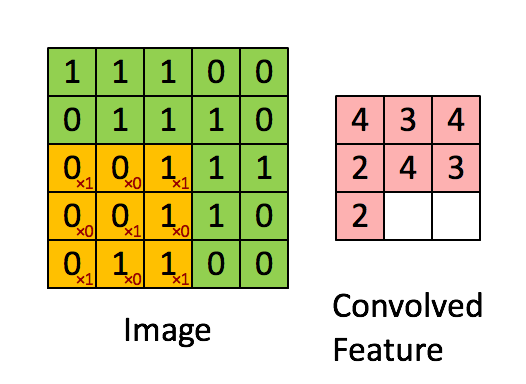
\includegraphics[width=0.5\textwidth]{figures/Convolution_schematic.gif}
  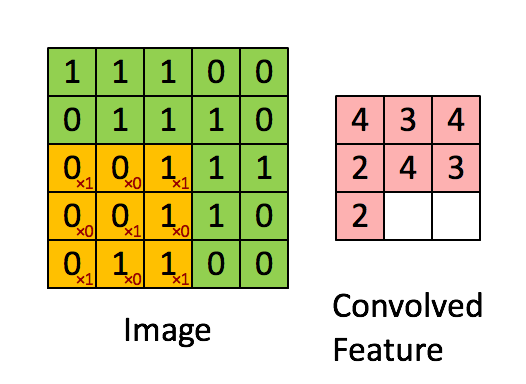
\includegraphics[width=0.5\textwidth]{figures/Convolution_schematic}
  %\caption{}\label{fig:step1}
\end{figure}

% σ \sigma
\cnt{Formally, given some large $r \times c$ images $x_{large}$, we first train a sparse autoencoder on small $a \times b$ patches xsmall sampled from these images, learning $k$ features $f = \sigma(W^{(1)}x_{small} + b^{(1)})$ (where $\sigma$ is the sigmoid function), given by the weights $W^{(1)}$ and biases $b^{(1)}$ from the visible units to the hidden units. For every $a \times b$ patch xs in the large image, we compute $f_s = \sigma (W^{(1)}x_s + b^{(1)})$, giving us $f_{convolved}$, a $k \times (r - a + 1) \times (c - b + 1)$ array of convolved features.}
    {假设给定了 $r \times c$ 的大尺寸图像,将其定义为 $x_{large}$。首先通过从大尺寸图像中抽取的 $a \times b$ 的小尺寸图像样本 $x_{small}$ 训练稀疏自编码,计算 $f = \sigma(W^{(1)}x_{small} + b^{(1)})$($\sigma$ 是一个 sigmoid 型函数)得到了 $k$ 个特征, 其中 $W^{(1)}$ 和 $b^{(1)}$ 是可视层单元和隐含单元之间的权重和偏差值。对于每一个 $a \times b$ 大小的小图像 xs,计算出对应的值 $f_s = \sigma (W^{(1)}x_s + b^{(1)})$,对这些 $f_{convolved}$ 值做卷积,就可以得到 $k \times (r - a + 1) \times (c - b + 1)$ 个卷积后的特征的矩阵。}
    {}


\cnt{In the next section, we further describe how to ``pool" these features together to get even better features for classification. }
    {在接下来的章节里,我们会更进一步描述如何把这些特征汇总到一起以得到一些更利于分类的特征。 }
    {}



\subsection{\cnt{Pooling}{池化}{}} \label{chp:pooling}

\subsubsection{\cnt{Pooling: Overview}{池化: 概述}{}}

\cnt{After obtaining features using convolution, we would next like to use them for classification. In theory, one could use all the extracted features with a classifier such as a softmax classifier, but this can be computationally challenging. Consider for instance images of size $96 \times 96$ pixels, and suppose we have learned 400 features over $8 \times 8$ inputs. Each convolution results in an output of size $(96 - 8 + 1) * (96 - 8 + 1) = 7921$, and since we have 400 features, this results in a vector of $89^2 * 400 = 3,168,400$ features per example. Learning a classifier with inputs having $3+$ million features can be unwieldy, and can also be prone to over-fitting.}
    {在通过卷积获得了特征 (features) 之后,下一步我们希望利用这些特征去做分类。理论上讲,人们可以用所有提取得到的特征去训练分类器,例如 softmax 分类器,但这样做面临计算量的挑战。例如:对于一个 $96 \times 96$ 像素的图像,假设我们已经学习得到了400个定义在$8 \times 8$输入上的特征,每一个特征和图像卷积都会得到一个 $(96 - 8 + 1) * (96 - 8 + 1) = 7921$ 维的卷积特征,由于有 400 个特征,所以每个样例 (example) 都会得到一个 $89^2 * 400 = 3,168,400$ 维的卷积特征向量。学习一个拥有超过 3 百万特征输入的分类器十分不便,并且容易出现过拟合 (over-fitting)。 }
    {}

\cnt{To address this, first recall that we decided to obtain convolved features because images have the ``stationarity" property, which implies that features that are useful in one region are also likely to be useful for other regions. Thus, to describe a large image, one natural approach is to aggregate statistics of these features at various locations. For example, one could compute the mean (or max) value of a particular feature over a region of the image. These summary statistics are much lower in dimension (compared to using all of the extracted features) and can also improve results (less over-fitting). We aggregation operation is called this operation \emph{pooling}, or sometimes \emph{mean pooling} or \emph{max pooling} (depending on the pooling operation applied).}
    {为了解决这个问题,首先回忆一下,我们之所以决定使用卷积后的特征是因为图像具有一种“静态性”的属性,这也就意味着在一个图像区域有用的特征极有可能在另一个区域同样适用。因此,为了描述大的图像,一个很自然的想法就是对不同位置的特征进行聚合统计,例如,人们可以计算图像一个区域上的某个特定特征的平均值 (或最大值)。这些概要统计特征不仅具有低得多的维度 (相比使用所有提取得到的特征),同时还会改善结果(不容易过拟合)。这种聚合的操作就叫做池化 (pooling),有时也称为平均池化或者最大池化 (取决于计算池化的方法)。 }
    {}

\cnt{The following image shows how pooling is done over 4 non-overlapping regions of the image.}
    {下图显示池化如何应用于一个图像的四块不重合区域。}
    {}

\begin{figure}[ht] \centering
  %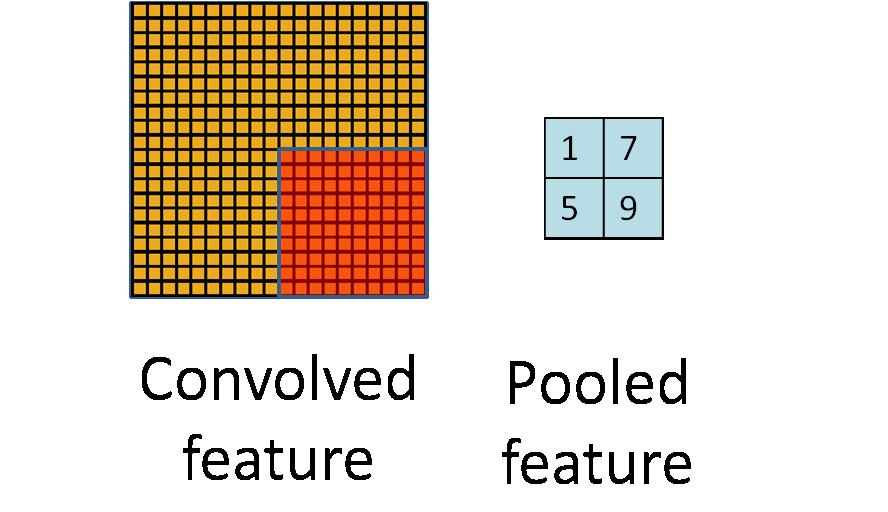
\includegraphics[width=0.5\textwidth]{figures/Pooling_schematic.gif}
  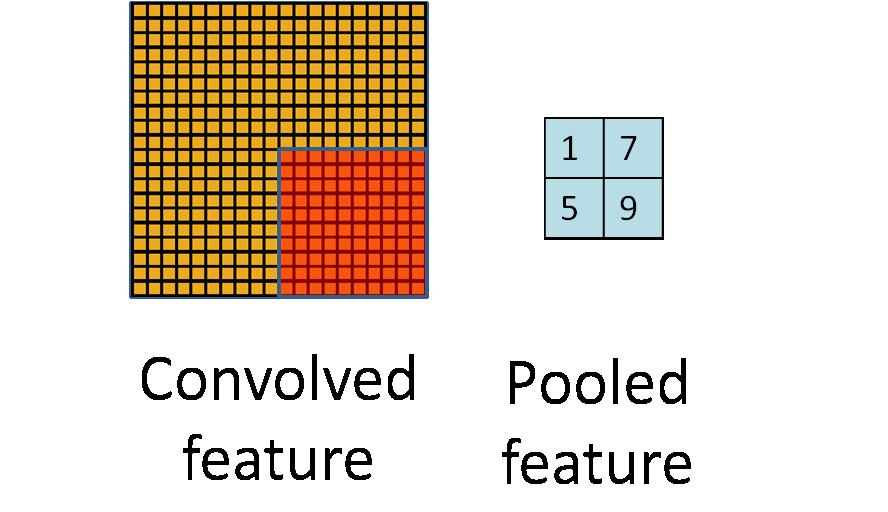
\includegraphics[width=0.5\textwidth]{figures/Pooling_schematic.png}
  %\caption{}\label{fig:step1}
\end{figure}

\subsubsection{\cnt{Pooling for Invariance}{池化的不变性}{}}

\cnt{If one chooses the pooling regions to be contiguous areas in the image and only pools features generated from the same (replicated) hidden units. Then, these pooling units will then be \emph{translation invariant}. This means that the same (pooled) feature will be active even when the image undergoes (small) translations. Translation-invariant features are often desirable; in many tasks (e.g., object detection, audio recognition), the label of the example (image) is the same even when the image is translated. For example, if you were to take an MNIST digit and translate it left or right, you would want your classifier to still accurately classify it as the same digit regardless of its final position.}
    {如果人们选择图像中的连续范围作为池化区域,并且只是池化相同(重复)的隐藏单元产生的特征,那么,这些池化单元就具有平移不变性 (translation invariant)。这就意味着即使图像经历了一个小的平移之后,依然会产生相同的 (池化的) 特征。在很多任务中 (例如物体检测、声音识别),我们都更希望得到具有平移不变性的特征,因为即使图像经过了平移,样例(图像)的标记仍然保持不变。例如,如果你处理一个MNIST数据集的数字,把它向左侧或右侧平移,那么不论最终的位置在哪里,你都会期望你的分类器仍然能够精确地将其分类为相同的数字。 }
    {}


\cnt{}
    {(*MNIST 是一个手写数字库识别库: \url{http://yann.lecun.com/exdb/mnist/})}
    {}

\subsubsection{\cnt{Formal description}{形式化描述}{}}

\cnt{Formally, after obtaining our convolved features as described earlier, we decide the size of the region, say $m \times n$ to pool our convolved features over. Then, we divide our convolved features into disjoint $m \times n$ regions, and take the mean (or maximum) feature activation over these regions to obtain the pooled convolved features. These pooled features can then be used for classification.}
    {形式上,在获取到我们前面讨论过的卷积特征后,我们要确定池化区域的大小(假定为$m \times n$),来池化我们的卷积特征。那么,我们把卷积特征划分到数个大小为 $m \times n$ 的不相交区域上,然后用这些区域的平均(或最大)特征来获取池化后的卷积特征。这些池化后的特征便可以用来做分类。 }
    {}

\subsection{\cnt{Exercise:Convolution and Pooling}{练习:卷积和池化}{}} \label{chp:execconvpool}

\cnt{In this exercise you will use the features you learned on $8 \times 8$ patches sampled from images from the STL-10 dataset in the earlier exercise on linear decoders(\ref{chp:execcolorfeaturesparseautoenc}) for classifying images from a reduced STL-10 dataset applying convolution(\ref{chp:convfeatureextract}) and pooling(\ref{chp:pooling}). The reduced STL-10 dataset comprises $64 \times 64$ images from 4 classes (airplane, car, cat, dog).}
    {}
    {}

\cnt{In the file \href{http://ufldl.stanford.edu/wiki/resources/cnn_exercise.zip}{cnn\_exercise.zip} we have provided some starter code. You should write your code at the places indicated ``YOUR CODE HERE" in the files.}
    {}
    {}

\cnt{For this exercise, you will need to modify cnnConvolve.m and cnnPool.m.}
    {}
    {}

\subsubsection{\cnt{Dependencies}{}{}}

\cnt{The following additional files are required for this exercise:}
    {}
    {}
\begin{itemize}
  \item \href{http://ufldl.stanford.edu/wiki/resources/stlSubset.zip}{A subset of the STL10 Dataset (stlSubset.zip)}
  \item \href{http://ufldl.stanford.edu/wiki/resources/cnn_exercise.zip}{Starter Code (cnn\_exercise.zip)}
\end{itemize}

\cnt{You will also need:}
    {}
    {}
\begin{itemize}
  \item \texttt{sparseAutoencoderLinear.m} or your saved features from Exercise:Learning color features with Sparse Autoencoders (\ref{chp:execcolorfeaturesparseautoenc})
  \item \texttt{feedForwardAutoencoder.m} (and related functions) from Exercise:Self-Taught Learning (\ref{chp:execselftaughtlearn})
  \item \texttt{softmaxTrain.m} (and related functions) from Exercise:Softmax Regression (\ref{chp:execsoftmaxreg})
\end{itemize}

\emph{
\cnt{If you have not completed the exercises listed above, we strongly suggest you complete them first.}
    {}
    {}
}

\subsubsection{\cnt{Step 1: Load learned features}{}{}}


\cnt{In this step, you will use the features from Exercise:Learning color features with Sparse Autoencoders(\ref{chp:execcolorfeaturesparseautoenc}). If you have completed that exercise, you can load the color features that were previously saved. To verify that the features are good, the visualized features should look like the following: }
    {}
    {}


%duplicated figure
\begin{figure}[ht] \centering
  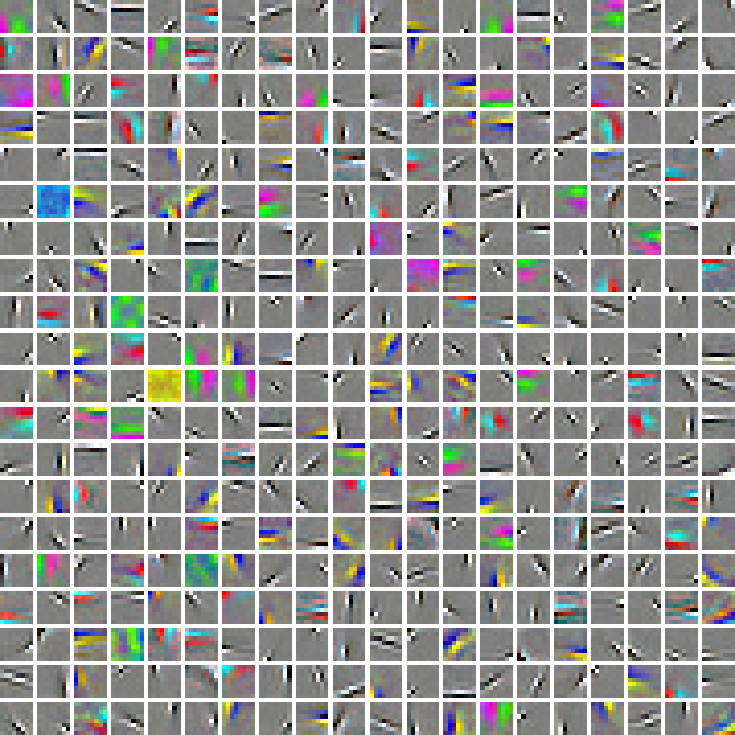
\includegraphics[width=0.5\textwidth]{figures/CNN_Features_Good.png}
  %\caption{}\label{fig:step1}
\end{figure}


\subsubsection{\cnt{Step 2: Implement and test convolution and pooling}{}{}}

\cnt{In this step, you will implement convolution and pooling, and test them on a small part of the data set to ensure that you have implemented these two functions correctly. In the next step, you will actually convolve and pool the features with the STL-10 images.}
    {}
    {}


\subsubsection{\cnt{Step 2a: Implement convolution}{}{}}

\cnt{Implement convolution, as described in feature extraction using convolution(\ref{chp:convfeatureextract}), in the function cnnConvolve in cnnConvolve.m. Implementing convolution is somewhat involved, so we will guide you through the process below.}
    {}
    {}

\cnt{First, we want to compute $\sigma(Wx_{(r,c)} + b)$ for all \emph{valid} $(r,c)$ (\emph{valid} meaning that the entire $8 \times 8$ patch is contained within the image; this is as opposed to a \emph{full} convolution, which allows the patch to extend outside the image, with the area outside the image assumed to be 0), where $W$ and $b$ are the learned weights and biases from the input layer to the hidden layer, and $x_{(r,c)}$ is the $8 \times 8$ patch with the upper left corner at $(r,c)$. To accomplish this, one naive method is to loop over all such patches and compute $\sigma(Wx_{(r,c)} + b)$ for each of them; while this is fine in theory, it can very slow. Hence, we usually use Matlab's built in convolution functions, which are well optimized.}
    {}
    {}

\cnt{Observe that the convolution above can be broken down into the following three small steps. First, compute $Wx_{(r,c)}$ for all $(r,c)$. Next, add b to all the computed values. Finally, apply the sigmoid function to the resulting values. This doesn't seem to buy you anything, since the first step still requires a loop. However, you can replace the loop in the first step with one of MATLAB's optimized convolution functions, \texttt{conv2}, speeding up the process significantly.}
    {}
    {}

\cnt{However, there are two important points to note in using \texttt{conv2}.}
    {}
    {}

\cnt{First, \texttt{conv2} performs a 2-D convolution, but you have 5 ``dimensions" - image number, feature number, row of image, column of image, and (color) channel of image - that you want to convolve over. Because of this, you will have to convolve each feature and image channel separately for each image, using the row and column of the image as the 2 dimensions you convolve over. This means that you will need three outer loops over the image number \texttt{imageNum}, feature number \texttt{featureNum}, and the channel number of the image channel. Inside the three nested for-loops, you will perform a \texttt{conv2} 2-D convolution, using the weight matrix for the \texttt{featureNum}-th feature and \texttt{channel}-th channel, and the image matrix for the \texttt{imageNum}-th image.}
    {}
    {}

\cnt{Second, because of the mathematical definition of convolution, the feature matrix must be ``flipped" before passing it to \texttt{conv2}. The following implementat}
    {}
    {}

%\notes{
\cnt{Implementation tip: Using \texttt{conv2} and \texttt{convn}}
    {}
    {}

\cnt{Because the mathematical definition of convolution involves ``flipping" the matrix to convolve with (reversing its rows and its columns), to use MATLAB's convolution functions, you must first ``flip" the weight matrix so that when MATLAB ``flips" it according to the mathematical definition the entries will be at the correct place. For example, suppose you wanted to convolve two matrices \texttt{image} (a large image) and \texttt{W} (the feature) using \texttt{conv2(image, W)}, and \texttt{W} is a $3 \times 3$ matrix as below:}
    {}
    {}
$$
W = \begin{pmatrix} 1 & 2 & 3 \\ 4 & 5 & 6 \\ 7 & 8 & 9 \\ \end{pmatrix}
$$

\cnt{If you use \texttt{conv2(image, W)}, MATLAB will first ``flip" \texttt{W}, reversing its rows and columns, before convolving \texttt{W} with \texttt{image}, as below:}
    {}
    {}

$$
\begin{pmatrix} 1 & 2 & 3 \\ 4 & 5 & 6 \\ 7 & 8 & 9 \\ \end{pmatrix} \xrightarrow{flip} \begin{pmatrix} 9 & 8 & 7 \\ 6 & 5 & 4 \\ 3 & 2 & 1 \\ \end{pmatrix}
$$

\cnt{If the original layout of \texttt{W} was correct, after flipping, it would be incorrect. For the layout to be correct after flipping, you will have to flip W before passing it into \texttt{conv2}, so that after MATLAB flips \texttt{W} in \texttt{conv2}, the layout will be correct. For \texttt{conv2}, this means reversing the rows and columns, which can be done with flipud and fliplr, as shown below:}
    {}
    {}

\begin{lstlisting}[language=matlab]
% Flip W for use in conv2
W = flipud(fliplr(W));
\end{lstlisting}

%} % notes

\cnt{Next, to each of the \texttt{convolvedFeatures}, you should then add \texttt{b}, the corresponding bias for the \texttt{featureNum}-th feature.}
    {}
    {}

\cnt{However, there is one additional complication. If we had not done any preprocessing of the input patches, you could just follow the procedure as described above, and apply the sigmoid function to obtain the convolved features, and we'd be done. However, because you preprocessed the patches before learning features on them, you must also apply the same preprocessing steps to the convolved patches to get the correct feature activations.}
    {}
    {}

\cnt{In particular, you did the following to the patches:}
    {}
    {}

\begin{itemize}
  \item subtract the mean patch, \texttt{meanPatch} to zero the mean of the patches
  \item ZCA whiten using the whitening matrix \texttt{ZCAWhite}.
\end{itemize}

\cnt{These same three steps must also be applied to the input image patches.}
    {}
    {}

\cnt{Taking the preprocessing steps into account, the feature activations that you should compute is $\sigma(W(T(x-\bar{x})) + b)$, where $T$ is the whitening matrix and $\bar{x}$ is the mean patch. Expanding this, you obtain $\sigma(WTx - WT\bar{x} + b)$, which suggests that you should convolve the images with WT rather than W as earlier, and you should add $(b - WT\bar{x})$, rather than just $b$ to \texttt{convolvedFeatures}, before finally applying the sigmoid function.}
    {}
    {}


\subsubsection{\cnt{Step 2b: Check your convolution}{}{}}


\cnt{We have provided some code for you to check that you have done the convolution correctly. The code randomly checks the convolved values for a number of (feature, row, column) tuples by computing the feature activations using \texttt{feedForwardAutoencoder} for the selected features and patches directly using the sparse autoencoder.}
    {}
    {}


\subsubsection{\cnt{Step 2c: Pooling}{}{}}



\cnt{Implement pooling in the function \texttt{cnnPool} in \texttt{cnnPool.m}. You should implement mean pooling (i.e., averaging over feature responses) for this part.}
    {}
    {}


\subsubsection{\cnt{Step 2d: Check your pooling}{}{}}



\cnt{We have provided some code for you to check that you have done the pooling correctly. The code runs \texttt{cnnPool} against a test matrix to see if it produces the expected result.}
    {}
    {}


\subsubsection{\cnt{Step 3: Convolve and pool with the dataset}{}{}}


\cnt{In this step, you will convolve each of the features you learned with the full $64 \times 64$ images from the STL-10 dataset to obtain the convolved features for both the training and test sets. You will then pool the convolved features to obtain the pooled features for both training and test sets. The pooled features for the training set will be used to train your classifier, which you can then test on the test set.}
    {}
    {}

\cnt{Because the convolved features matrix is very large, the code provided does the convolution and pooling 50 features at a time to avoid running out of memory.}
    {}
    {}


\subsubsection{\cnt{Step 4: Use pooled features for classification}{}{}}

\cnt{In this step, you will use the pooled features to train a softmax classifier to map the pooled features to the class labels. The code in this section uses \texttt{softmaxTrain} from the softmax exercise to train a softmax classifier on the pooled features for 500 iterations, which should take around a few minutes.}
    {}
    {}


\subsubsection{\cnt{Step 5: Test classifier}{}{}}

\cnt{Now that you have a trained softmax classifier, you can see how well it performs on the test set. These pooled features for the test set will be run through the softmax classifier, and the accuracy of the predictions will be computed. You should expect to get an accuracy of around 80\%.}
    {}
    {}

